\section{利用CSS格式化XML}

\begin{frame}[fragile]{CH5 利用CSS格式化XML}
\begin{figure}
    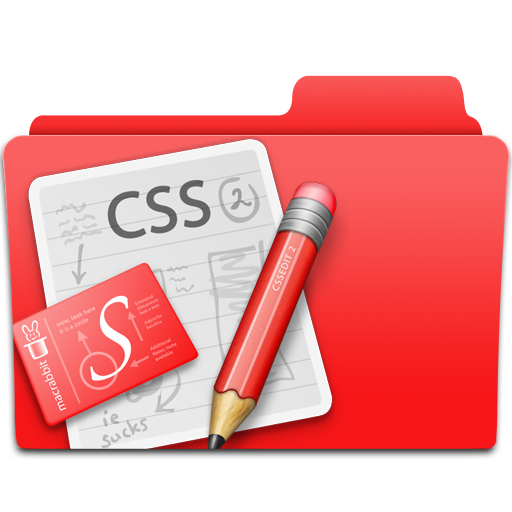
\includegraphics[width=0.5\textwidth]{figure/css.png}
\end{figure}
\end{frame}

\begin{frame}[fragile]{本章学习目标}
\begin{easylist} \easyitem
& 掌握CSS与XML、HTML的关联方式
& 掌握CSS的常见选择器,理解CSS的属性继承与覆盖原则
& 掌握CSS的颜色、字体和文本属性以及CSS的盒状模型
\end{easylist}
\end{frame}

\begin{frame}[fragile]{目录}
\begin{easylist} \easyitem
& 什么是CSS
& 关联CSS的方法
& CSS语法基础
&& CSS基本语法
&& CSS选择器
&& 继承与覆盖
& CSS重要属性
&& 颜色属性
&& 字体属性
&& 文本属性
&& 盒状模型相关属性
&& 可视格式化模型相关属性
\end{easylist}
\end{frame}


\subsection{5.1 什么是CSS}

\begin{frame}[fragile]{5.1 什么是CSS}
\begin{shaded}
CSS(Cascading Style Sheets),又称为层叠样式表或级联样式表,可以实现对页面布局、字体、颜色、背景和其他图文效果的精准控制,在XML和HTML的呈现中得到了广泛使用。
\end{shaded}

\begin{easylist} \easyitem
& CSS的优点
& CSS的发展历史
&& CSS1
&& CSS2, CSS 2.1
&& CSS 3
\end{easylist}
\end{frame}


\subsection{5.2 关联CSS的方法}

\begin{frame}[fragile]{5.2 关联CSS的方法}
\begin{easylist} \easyitem
& 与传统网页的关联方式
& \em{与XML的关联方式}
\end{easylist}
\end{frame}


\subsubsection{5.2.1 CSS与传统网页的关联方式}
\begin{frame}[fragile]{5.2.1 CSS与传统网页的关联方式}
\begin{easylist} \easyitem
& 独立引用方式
&& 通过HTML中的link标记链接外部独立的样式表文件。
& 网页内嵌方式
&& 在HTML的style标记对中嵌入样式代码块。
& 元素内联方式
&& 在HTML的一般元素上采用style属性直接设置元素的样式信息
\end{easylist}
\end{frame}


\begin{frame}[fragile, allowframebreaks]{示例}
\begin{lstlisting}[tabsize=8, basicstyle=\small\tt, language=HTML, caption=5-1.html]
<html>
    <head>
        <title>CSS DEMO</title>
        <meta http-equiv="Content-Type" content="text/html;charset=utf-8"/>
        <link rel="stylesheet" type="text/css" href="5-1.css"/>
        <style type="text/css">
            h1 {font-size:14pt;font-family:"Microsoft Yahie" 微软雅黑;}
        </style>
    </head>
    <body>
        <h1>图书列表</h1>
        <table>
            <tr>
                <td>ISBN</td><td>名称</td><td>出版社</td><td>价格</td>
            </tr>
            <tr>
                <td>978-7-115-21703-5</td>
                <td style="font-weight:bold;">Python高级编程</td>
                <td>人民邮电出版社</td>
                <td>45.00</td>
            </tr>
            <tr>
                <td>978-7-115-28282-8</td>
                <td>数学之美</td>
                <td>人民邮电出版社</td>
                <td>45.00</td>
            </tr>
            <tr>
                <td>978-7-5641-1139-7</td>
                <td>集体智慧编程(影印版)</td>
                <td>东南大学出版社</td>
                <td>58.00</td>
            </tr>
        </table>
    </body>
</html>
\end{lstlisting}

\begin{lstlisting}[tabsize=8, basicstyle=\small\tt, language=CSS,  caption=5-1.css]
td {
    border:1px solid blue;
}
\end{lstlisting}
\end{frame}


\begin{frame}[fragile]{示例}
\begin{figure}
    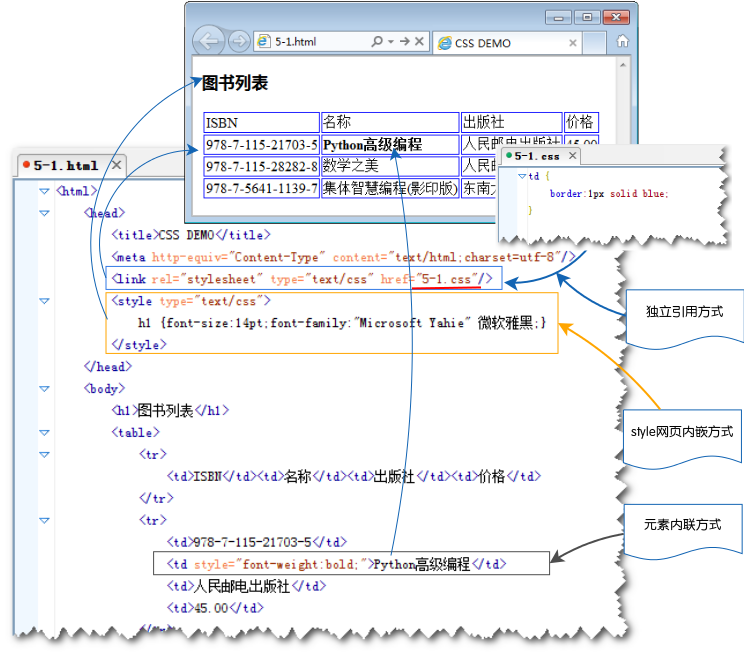
\includegraphics[width=0.75\textwidth]{figure/css-html-association.png}
\end{figure}
\end{frame}


\subsubsection{5.2.2 CSS与XML的关联方式}
\begin{frame}[fragile]{5.2.2 CSS与XML的关联方式}
\begin{easylist} \easyitem
& \em{通过<?xml-stylesheet?>处理指令实现关联}
& 非W3C规定,但得到主流浏览器的支持,成为事实标准
\end{easylist}
\end{frame}


\begin{frame}[fragile, allowframebreaks]{CSS与XML关联示例}
\begin{lstlisting}[tabsize=8, basicstyle=\small\tt, language=CSS,  caption=books.css]
book {display:block; margin:5px;}

title {   width:200px; 
           border: 1px solid gray;
           display:inline-block;
           padding:2px;
           padding-left:10px;
}

price { width:50px; 
           border: 1px solid gray;
           display:inline-block;
           padding:2px;
}

press { width:200px; 
           border: 1px solid gray; 
           display:inline-block;
           padding:2px;
}

authors, pages, description, cover {display: none;}
\end{lstlisting}

\begin{lstlisting}[tabsize=8, basicstyle=\small\tt, language=XML,  caption=books.xml]
<?xml version="1.0"?>
<?xml-stylesheet type="text/css" href="books.css"?>
<books>
    <book isbn="978-1449319793" id="b1">
        <title lang="EN">Python for Data Analysis</title>
        <price currency="dollar">25.40</price>
        <authors>
            <author>Wes McKinney</author>
        </authors>
        <press>OReilly Media</press>
        <pages>470</pages>
        <description>Python for Data Analysis...</description>
        <cover>book-python.jpg</cover>
    </book>
    <book isbn="978-7-115-28282-8" id="b2">
        <title lang="CHN">数学之美</title>
        <price>45.00</price>
        <authors>
            <author>吴军</author>
        </authors>
        <press>人民邮电出版社</press>
        <pages>304</pages>
        <description>读了“数学之美”,才发现大学时...</description>
        <cover>book-math.jpg</cover>
    </book>
</books>
\end{lstlisting}
\end{frame}


\subsection{5.3 CSS语法基础}
\begin{frame}[fragile]{5.3 CSS语法基础}
\begin{easylist} \easyitem
& CSS基本语法
& CSS选择器
& 继承与覆盖
\end{easylist}
\end{frame}

\subsubsection{5.3.1 CSS基本语法}
\begin{frame}[fragile, allowframebreaks]{5.3.1 CSS基本语法}
\begin{easylist} \easyitem
& 选择器 + 规则声明
& 形式:选择符 \{属性名: 属性值[; 属性名: 属性值]…\}
\begin{figure}
    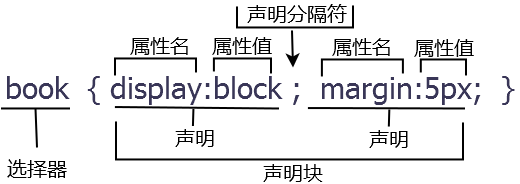
\includegraphics[width=0.75\textwidth]{figure/css-rule.png}
\end{figure}
&& 选择符(selector)
&&& 被施加样式的元素标记名(tag)、类([tag].class)或标识符([tag]\#id)等
&& 属性名称
&&& 表示颜色、字体等需要指定样式的名称
&& 属性值
&&& 表示属性具体的取值,如颜色取red,字体大小取12pt等
&& 英文冒号和分号作分隔
\end{easylist}
\end{frame}


\subsubsection{5.3.2 CSS选择器}
\begin{frame}[fragile]{5.3.2 CSS选择器}
\begin{easylist} \easyitem
& 元素选择器
& ID选择器
& 属性选择器
& 类选择器
& 通用选择器
& 分组选择器
& 后代选择器
\end{easylist}
\end{frame}


\begin{frame}[fragile]{元素选择器}
\begin{easylist} \easyitem
& 以元素名称作为选择器的表示方式,选择文档中的指定元素,是最常见的CSS选择方式
& 例子
\begin{lstlisting}[tabsize=8, basicstyle=\small\tt, language=CSS, numbers=none]
title {color: blue;}
\end{lstlisting}
\end{easylist}
\end{frame}


\begin{frame}[fragile]{ID选择器}
\begin{easylist} \easyitem
& 选择文档中具有特定id的元素
&& 在通过在id值前面附加字符“\#”作为选择器的表示方式
& 例子
\begin{lstlisting}[tabsize=8, basicstyle=\small\tt, language=CSS, numbers=none]
#b1 {color: red;}
\end{lstlisting}
\end{easylist}
\end{frame}


\begin{frame}[fragile]{属性选择器}
\begin{easylist} \easyitem
& 选择具有某个属性的元素集合
&& 将具有属性名称为lang的title元素的字体颜色设为橙色:
\begin{lstlisting}[tabsize=8, basicstyle=\small\tt, language=CSS, numbers=none]
title[lang] {color: orange;}
\end{lstlisting}
&& 将元素名称更改为星号可选择具有特定属性名称的任意元素即可
\begin{lstlisting}[tabsize=8, basicstyle=\small\tt, language=CSS, numbers=none]
*[isbn] {color:green;}
\end{lstlisting}
&& 选择具有特定属性名称和属性值的元素集合
\begin{lstlisting}[tabsize=8, basicstyle=\small\tt, language=CSS, numbers=none]
title[lang="CHN"] {color: red;}
\end{lstlisting}
\end{easylist}
\end{frame}


\begin{frame}[fragile]{类选择器}
\begin{easylist} \easyitem
& 选择具有特性class属性的元素集合,应用于HTML
& 例子
\begin{lstlisting}[tabsize=8, basicstyle=\small\tt, language=HTML, numbers=none]
<h1 class="important">这是重要标题</h1>
<p class="important">这是重要段落</p>
\end{lstlisting}
\begin{lstlisting}[tabsize=8, basicstyle=\small\tt, language=CSS, numbers=none]
.important{color: red;}
\end{lstlisting}
\end{easylist}
\end{frame}


\begin{frame}[fragile]{通用选择器}
\begin{easylist} \easyitem
& 星号“*”,匹配文档树中任何类型的元素名
& 例如:
\begin{lstlisting}[tabsize=8, basicstyle=\small\tt, language=CSS, numbers=none]
* {color: blue;}
\end{lstlisting}
& 非单独出现的通用选择器可以省略
\begin{lstlisting}[tabsize=8, basicstyle=\small\tt, language=CSS, numbers=none]
*[lang="CHN"] {color: red;} 等价于 [lang="CHN"] {color: red;}
*#b1 {color: red;} 等价于 #b1 {color: red;}
\end{lstlisting}
\end{easylist}
\end{frame}


\begin{frame}[fragile]{分组选择器}
\begin{easylist} \easyitem
& 一次选择多个元素
& 例子
\begin{lstlisting}[tabsize=8, basicstyle=\small\tt, language=CSS, numbers=none]
title, press {color: red;}
\end{lstlisting}
\end{easylist}
\end{frame}


\begin{frame}[fragile]{后代选择器}
\begin{easylist} \easyitem
& 把选中的元素限定在某些特定的文档结构中
& 例子
\begin{lstlisting}[tabsize=8, basicstyle=\small\tt, language=CSS, numbers=none]
#b1 title {color: blue;}
\end{lstlisting}
&& 将选中具有ID属性值为b1的元素内部的所有title子元素,并将其颜色设为蓝色
&& 后代选择器可选中任意符合选择器要求的后代元素
& 子元素选择器
&& 限定子元素
\begin{lstlisting}[tabsize=8, basicstyle=\small\tt, language=CSS, numbers=none]
book > title {color: blue;}
\end{lstlisting}
\end{easylist}
\end{frame}


\subsubsection{5.3.3 CSS的继承与覆盖}
\begin{frame}[fragile]{5.3.3 CSS的继承与覆盖}
\begin{easylist} \easyitem
& 属性继承
&& 子元素自动采用父元素中指定的样式作为本身的默认样式
& 属性覆盖
&& 一个元素最近指定的样式属性会覆盖之前指定的样式属性
\end{easylist}
\end{frame}


\begin{frame}[fragile]{支持继承的CSS属性}
\begin{easylist} \easyitem
& color
& font及相关属性
& letter-spacing
& line-height
& list-style及相关的属性
& text相关属性
& ...
\end{easylist}
\end{frame}


\begin{frame}[fragile]{不支持继承的CSS属性}
\begin{easylist} \easyitem
& background及相关属性
& border 及相关属性
& display
& float 和 clear
& margin及相关属性
& ...
\end{easylist}
\end{frame}


\begin{frame}[fragile]{属性覆盖原则-1}
\begin{easylist} \easyitem
& 当因继承而发生样式冲突时,最近祖先的样式将覆盖更远祖先的样式
\begin{lstlisting}[tabsize=8, basicstyle=\small\tt, language=CSS, numbers=none]
books {color:blue; }
book {color:red; }
\end{lstlisting}
\end{easylist}
\end{frame}


\begin{frame}[fragile]{属性覆盖原则-2}
\begin{easylist} \easyitem
& 当直接指定的样式与继承样式冲突时,将采用直接指定的样式
\begin{lstlisting}[tabsize=8, basicstyle=\small\tt, language=CSS, numbers=none]
books {color:blue; }
book {color:red; }
title {color:orange; }
\end{lstlisting}
\end{easylist}
\end{frame}


\begin{frame}[fragile]{属性覆盖原则-3}
\begin{easylist} \easyitem
& 当直接指定的样式发生冲突时,采用权重高者的样式
\begin{lstlisting}[tabsize=8, basicstyle=\small\tt, language=CSS, numbers=none]
book {color:blue; }
#b1 {color:red; }
\end{lstlisting}
&& ID选择器的权重高于元素选择器,因此,ID为b1的图书内容将以红色字体显示
\end{easylist}
\end{frame}


\begin{frame}[fragile]{属性覆盖原则-4}
\begin{easylist} \easyitem
& 当样式权重相同时,采用最后指定的样式
\begin{lstlisting}[tabsize=8, basicstyle=\small\tt, language=CSS, numbers=none]
book title[lang] {color: blue;}
book[isbn] title {color: red;}
\end{lstlisting}
\end{easylist}
\end{frame}


\begin{frame}[fragile]{属性覆盖原则-5}
\begin{easylist} \easyitem
& !important的样式属性不被覆盖
\begin{lstlisting}[tabsize=8, basicstyle=\small\tt, language=CSS, numbers=none]
book {color:blue !important; }
#b1 {color:red; }
\end{lstlisting}
&& 虽然ID选择器的权重高于元素选择器,但由于book元素选择器中的样式指定了!important,从而使ID为b1的图书元素强制显示为蓝色
\end{easylist}
\end{frame}



\subsection{5.4 CSS重要属性}
\begin{frame}[fragile]{5.4 CSS重要属性}
\begin{easylist} \easyitem
& 颜色属性
& 字体属性
& 文本属性
& 盒状模型相关属性
& 可视格式化模型相关属性
\end{easylist}
\end{frame}


\subsubsection{5.4.1 颜色属性}
\begin{frame}[fragile]{5.4.1 颜色属性}
\begin{easylist} \easyitem
& 名称表示方式
&& black, white, blue, yellow, red, ...
& RGB表示方式
&& \#rrggbb
&&& 两位十六进制数字(00~FF)分别表示红绿蓝三种颜色的分量取值, 如:\#FF0000
&& \#rgb 
&&& 等价于 \#rrggbb,如:\#F00
&& RGB(r, g, b)
&&& 以十进制指定红绿蓝颜色分量值,如: RGB(255,0,0)
&& RGB(r\%, g\%, b\%)
&&& 用百分比表示红绿蓝分量比重,如: RGB(100\%, 0\%, 0\%)
\end{easylist}
\end{frame}


\begin{frame}[fragile]{颜色名称和RGB值}
\begin{figure}
    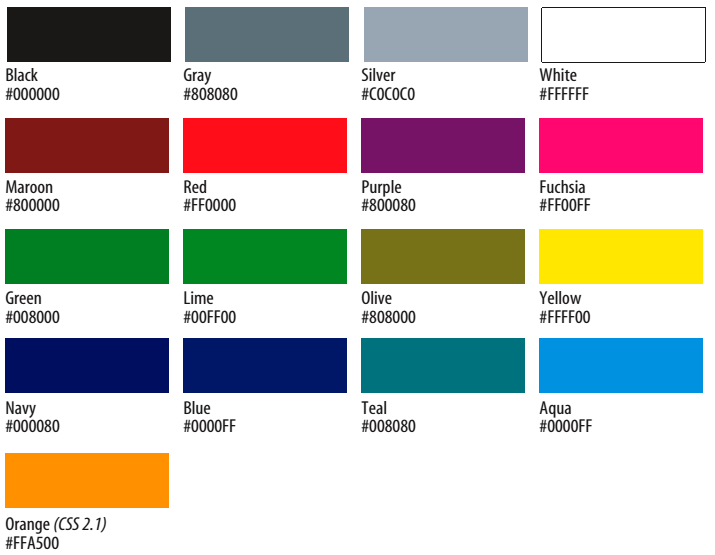
\includegraphics[width=0.75\textwidth]{figure/css-colors.png}
\end{figure}
\end{frame}


\begin{frame}[fragile]{颜色示例}
\begin{lstlisting}[tabsize=8, basicstyle=\small\tt, language=CSS]
book {display:block; margin:5px; }
title { width:200px; border: 1px solid gray;
        display:inline-block;padding:2px;padding-left:10px;}
price { width:50px; border: 1px solid gray;
        display:inline-block;padding:2px;}
press { width:200px; border: 1px solid gray;
        display:inline-block;padding:2px;}
authors, pages, description, cover {display: none;}

title {color: blue;}
price {color: #FFA500; }
press {color:RGB(255, 0, 0);}
\end{lstlisting}
\end{frame}


\begin{frame}[fragile]{浏览器中的呈现效果}
\begin{figure}
    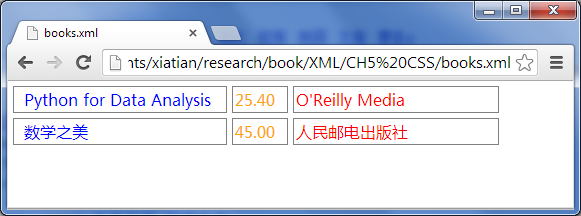
\includegraphics[width=0.75\textwidth]{figure/css-color-demo.png}
\end{figure}
\end{frame}


\subsubsection{5.4.2 字体属性}
\begin{frame}[fragile]{5.4.2 字体属性}
\begin{easylist} \easyitem
& 字体族font-family
& 字体风格font-style
&& normal | italic | oblique | inherit
& 字体变体font-variant
&& normal | small-caps | inherit
& 字体粗细font-weight
&& normal | bold | bolder | lighter | 100 | 200 | 300 | 400 | 500 | 600 | 700 | 800 | 900 | inherit
& 字体大小font-size
\end{easylist}
\end{frame}


\begin{frame}[fragile]{font-family}
\begin{easylist} \easyitem
& 定义文本所使用的字体族
&& 字体族由一系列相关字体组成,如微软雅黑字体作为一个字体族会包括大小、粗体、斜体等不同显示效果的字体
& family-name(字体族名称)
&& 通常所说的“字体”,如“Arial”、“Times New Roman”、“宋体”、“微软雅黑”等
& generic family(族类名称)
&& 一组具有统一外观的字体族,它包含的范围比family-name更大,可看作是一组具有某些共同特点的family-name的集合
\end{easylist}
\end{frame}


\begin{frame}[fragile]{Generic Family: Serif、Sans-serif and Monospace}
\begin{figure}
    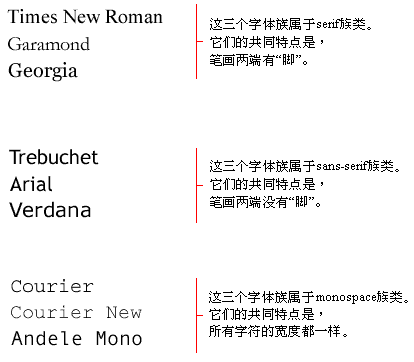
\includegraphics[width=0.75\textwidth]{figure/css-generic-family.png}
\end{figure}
\end{frame}


\begin{frame}[fragile, allowframebreaks]{font-size}
\begin{easylist} \easyitem
& 绝对大小<absolute-size> 
&& xx-small | x-small | small | medium | large | x-large | xx-large
& 相对大小<relative-size>
&&  larger | smaller 
& 指定长度<length>
&& 相对长度单位:
&&& em: the ‘font-size’ of the relevant font
&&& ex: the ‘x-height’ of the relevant font
&&& \em{px: pixels, 像素,相对于显示设备的最小显示单位}
&& 绝对长度单位:
&&& in: inches,英寸,一英寸约等于2.54厘米
&&& cm: centimeters,厘米
&&& mm: millimeters,毫米
&&& \em{pt: pofints,等于1/72英寸}
&&& pc: picas,等于12 points
& 百分比<percentage>
&& 相对于继承的字体大小的百分比
\end{easylist}
\end{frame}


\begin{frame}[fragile, allowframebreaks]{例子}
\begin{lstlisting}[tabsize=8, basicstyle=\small\tt, language=CSS,  caption=books-font.css]
book {display:block; margin:5px; }
title { width:200px; border: 1px solid grey;
    display:inline-block;padding:2px;padding-left:10px;
}
price { width:50px; border: 1px solid grey;
    display:inline-block;padding:2px;
}
press { width:200px; border: 1px solid grey; 
    display:inline-block;padding:2px;
}
authors, pages, description, cover {display: none;}

book {font-family: “Times New Roman”, “微软雅黑”, Serif;}
title {font-weight:bold;}
press {font-variant:small-caps;}
book#b2 title {font-size: larger;}
book#b2 price {font-size: 10pt;}
\end{lstlisting}
\begin{figure}
    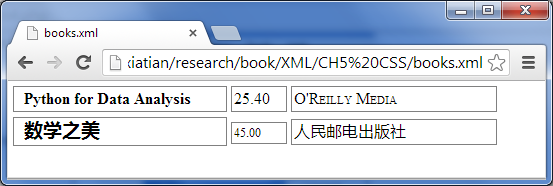
\includegraphics[width=0.75\textwidth]{figure/css-font-demo.png}
\end{figure}
\end{frame}



\begin{frame}[fragile, allowframebreaks]{font}
\begin{easylist} \easyitem
& 字体样式的简写方式
&& 顺序: font-style | font-variant | font-weight | font-size | font-family
& 以下两段代码等价:
\begin{lstlisting}[tabsize=8, basicstyle=\small\tt, language=CSS]
title {
    font-style: italic;
    font-weight: bold;
    font-size: 16px;
    font-family: arial, sans-serif;
}
\end{lstlisting}
\begin{lstlisting}[tabsize=8, basicstyle=\small\tt, language=CSS]
title { 
    font: italic bold 16px arial,sans-serif;
}
\end{lstlisting}
\end{easylist}
\end{frame}



\subsubsection{5.4.3 文本属性}
\begin{frame}[fragile, allowframebreaks]{5.4.3 文本属性}
\begin{easylist} \easyitem
& text-indent(文本缩进)
&& 设置文本块中首行文本的缩进或悬挂,缺省值为0(不缩进)
\begin{lstlisting}[tabsize=8, basicstyle=\small\tt, language=CSS, numbers=none]
title { text-indent: 3em; } 
\end{lstlisting}
&&& 例如将title元素内容缩进3个字

& text-align(文本对齐)
&& 设置文本段的对齐特性
&& 取值:
&&& left(左对齐)
&&& right(右对齐)
&&& center(居中)
&&& justify(两端撑满)
&&& inherit(继承)

& text-decoration(文本修饰)
&& 取值可以为:
&&& none(无修饰,为缺省值)
&&& underline(下划线)
&&& overline(上划线)
&&& line-through(删除线)
&&& blink(闪烁)
&&& inherit(继承)

& letter-spacing(字母间隔)和 word-spacing(词间隔)
&& 取值均可以为
&&& normal(缺省值)
&&& 指定长度
&&& inherit(继承)

& text-transform(文本转换)
&& 用于进行大小写转换
&&& capitalize——每个单词的首字母大写,其他字母不变
&&& uppercase——所有字母全大写
&&& lowercase——所有字母全小写
&&& none——不转换,使用默认值,为缺省值
&&& inherit——继承

& white-space(空白)
&& 设置对文本中对空白符的处理方法
&&& normal——收缩白空序列,自动换行,为缺省值
&&& pre——防止(prevent)白空序列收缩,保留白空符不变
&&& nowrap——收缩白空序列,但抑制换行
&&& pre-wrap——不收缩白空序列,在源文本的回车和换行处换行,并在需要的地方自动换行
&&& pre-line——收缩白空序列,在源文本的回车和换行处换行,并在需要的地方自动换行
\end{easylist}
\end{frame}


\begin{frame}[fragile, allowframebreaks]{例子}
\begin{lstlisting}[tabsize=8, basicstyle=\small\tt, language=CSS,  caption=books-font.css]
book {display:block; margin:5px; }
title { width:250px; border: 1px solid gray;
            display:inline-block;padding:2px;padding-left:10px;}
price { width:50px; border: 1px solid gray;
            display:inline-block;padding:2px;}
press { width:250px; border: 1px solid gray; 
            display:inline-block;padding:2px;}
authors, pages, description, cover {display: none;}

title {
            text-indent:1em; 
            text-decoration:underline;
            letter-spacing:0.1em;
}
press {
            text-align:center; 
            word-spacing:1cm;
            text-transform:uppercase;
}
\end{lstlisting}
\begin{figure}
    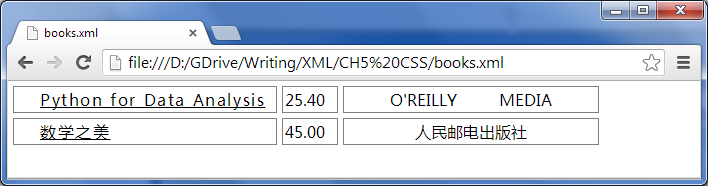
\includegraphics[width=0.75\textwidth]{figure/css-text-demo.png}
\end{figure}
\end{frame}



\subsubsection{5.4.4 盒状模型相关属性}
\begin{frame}[fragile]{5.4.4 盒状模型相关属性}
\begin{figure}
    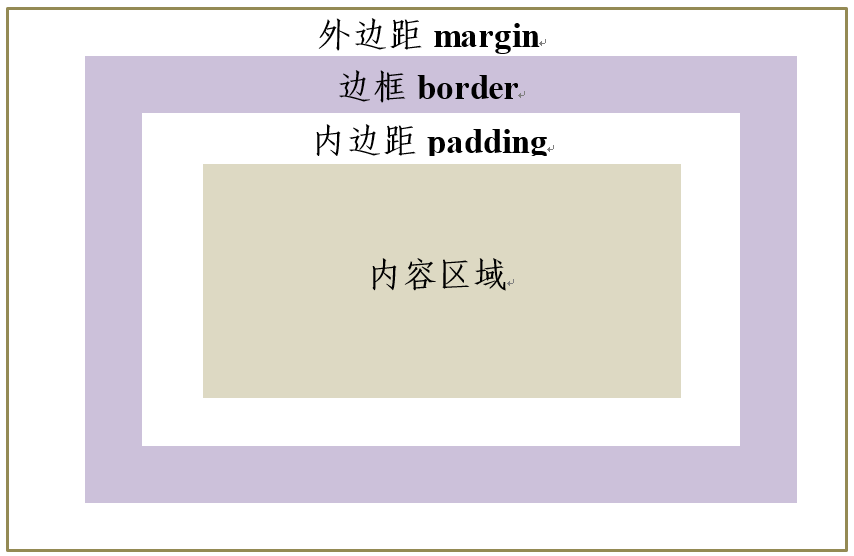
\includegraphics[width=0.60\textwidth]{figure/css-box-model.png}
\end{figure}
\begin{easylist} \easyitem
& 盒状模型
&& margin
&& padding
&& border
\end{easylist}
\end{frame}


\begin{frame}[fragile]{padding}
\begin{easylist} \easyitem
& 简写方式:直接指定一个数值
\begin{lstlisting}[tabsize=8, basicstyle=\small\tt, language=CSS, numbers=none]
title { padding:2px; } 
\end{lstlisting}
& 按照上、右、下、左的顺时针方向顺序分别设置各边的内边距
\begin{lstlisting}[tabsize=8, basicstyle=\small\tt, language=CSS, numbers=none]
title { padding: 2px 5% 5px 2%;}
\end{lstlisting}
& 分别设置
&& padding-top
&& padding-right
&& padding-bottom
&& padding-left
\end{easylist}
\end{frame}


\begin{frame}[fragile]{margin}
\begin{easylist} \easyitem
& 简写方式:直接指定一个数值
\begin{lstlisting}[tabsize=8, basicstyle=\small\tt, language=CSS, numbers=none]
book { margin: 10px;}
\end{lstlisting}
& 按照上、右、下、左的顺时针方向顺序分别设置各边的外边距
\begin{lstlisting}[tabsize=8, basicstyle=\small\tt, language=CSS, numbers=none]
book { margin: 5px 10px 5px 5%;}
\end{lstlisting}
& 分别设置
&& margin-top
&& margin-right
&& margin-bottom
&& margin-left
\end{easylist}
\end{frame}


\begin{frame}[fragile]{border}
\begin{easylist} \easyitem
& border-width
\begin{lstlisting}[tabsize=8, basicstyle=\small\tt, language=CSS, numbers=none]
title {border-width: medium;}
price {border-width: 2px;}
\end{lstlisting}

& border-color
\begin{lstlisting}[tabsize=8, basicstyle=\small\tt, language=CSS, numbers=none]
title {border-color: red;}
\end{lstlisting}

& border-style
\begin{lstlisting}[tabsize=8, basicstyle=\small\tt, language=CSS, numbers=none]
book {border-style: solid;}
\end{lstlisting}
\end{easylist}
\end{frame}



\begin{frame}[fragile]{border简写方式}
\begin{easylist} \easyitem
& 以下两段代码等价
\begin{lstlisting}[tabsize=8, basicstyle=\small\tt, language=CSS]
title {
    border-width: 2px;
    border-style: solid;
    border-color: red;
}
\end{lstlisting}
\begin{lstlisting}[tabsize=8, basicstyle=\small\tt, language=CSS, numbers=none]
title { border: 2px solid red;}
\end{lstlisting}
\end{easylist}
\end{frame}


\begin{frame}[fragile]{练习}
\begin{easylist} \easyitem
& 通过CSS控制“books.xml”显示效果,在“books.css”的基础上,满足以下要求:
&& title、price和press元素仅显示2个像素、灰色的实线下边框
&& 每行图书下面的外边距为15个像素
&& price元素的左侧内边距为20个像素
\end{easylist}
\end{frame}


\subsubsection{5.4.5 可视格式化模型相关属性}
\begin{frame}[fragile]{5.4.5 可视格式化模型相关属性}
\begin{easylist} \easyitem
& 可视格式化模型VFM: Visual Formatting Model
&& 每个元素会依据盒状模型生成0个或多个盒子
&& 盒子的布局由盒的尺寸和类型、定位方案、文档树中元素间的关系、以及外部信息所控制
&& 包括显示、高度、宽度、定位、文本方向等属性
\end{easylist}
\end{frame}


\begin{frame}[fragile]{display显示属性}
\begin{easylist} \easyitem
& display显示属性
&& 用于设置和改变元素所对应的盒子的显示类型
&& 元素既可以显示为独立的一块内容,即块元素
&& 也可以显示在一行中,即行内元素
\end{easylist}
\end{frame}


\begin{frame}[fragile]{display属性常见取值及作用}
\begin{table}[!hbp] 
\begin{tabular}{|l|l|}
\Xhline{1.3pt}
display属性取值 & 作用\\ \Xhline{1.3pt}
block & 使元素产生一个块状盒子,并换行\\ \hline
inline-block & 产生一个行内(inline)块状盒子,不强制换行\\ \hline
inline & 产生一个或多个行内盒子,缺省值\\ \hline
list-item & 产生一个主块和一个表项行内盒\\ \hline
none & 不产生盒子,即无布局效果\\ \hline
\end{tabular}
\end{table}
\end{frame}


\begin{frame}[fragile]{宽度和高度属性}
\begin{easylist} \easyitem
& 宽度属性width
&& 指定由块级元素和替换元素所生成的盒子的内容宽度
&& 取值可以为长度或百分比
& 高度属性height
&& 用于对元素盒子的高度进行限定,
&& 取值同样为长度值或百分比
& 例子
\begin{lstlisting}[tabsize=8, basicstyle=\small\tt, language=CSS, numbers=none]
title{height:30px; width:500px;}
\end{lstlisting}
&& 指定title元素的高度和宽度分别为30个像素和500个像素大小
\end{easylist}
\end{frame}



\begin{frame}
\begin{center}
    \Huge END
\end{center}
\begin{figure}
    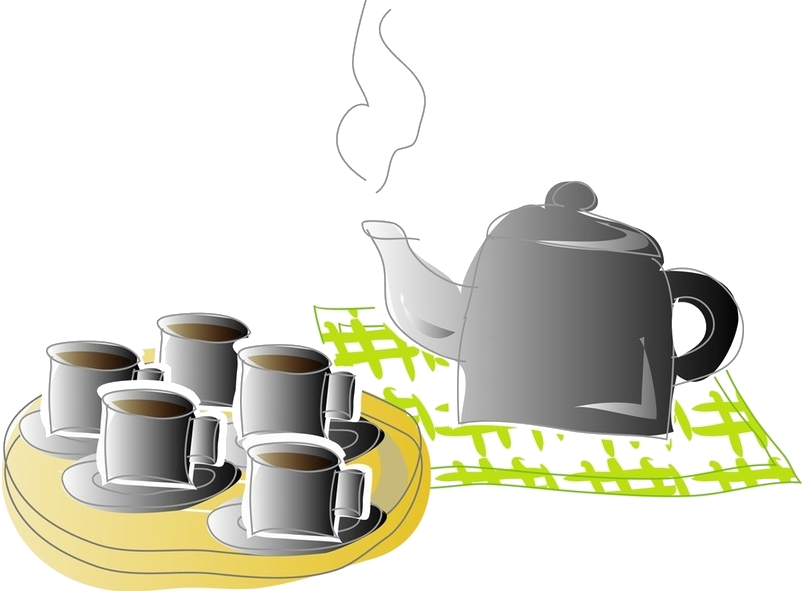
\includegraphics[width=0.75\textwidth]{figure/relax.png}
\end{figure}
\end{frame}
